\documentclass{article}
\usepackage[utf8]{inputenc}
\usepackage{graphicx}

\begin{document}

\Large{\title{\textbf{Proof of Concept}}}
\author{Bree Kelly} \date{}

\maketitle

\section*{Scoping Exercise}
\paragraph{} ~\\ \large
\noindent{\textbf{Elaboration 1}}
\newline \break
I want to take a passage of hieroglyphic text through the process of translation, using the Hieroglyphics Initiative as a digital tool.
\newline ~\\
For example, if I were to use the platform to assist me in translating the passage below from the Story of Sinuhe:
\paragraph{}~\\
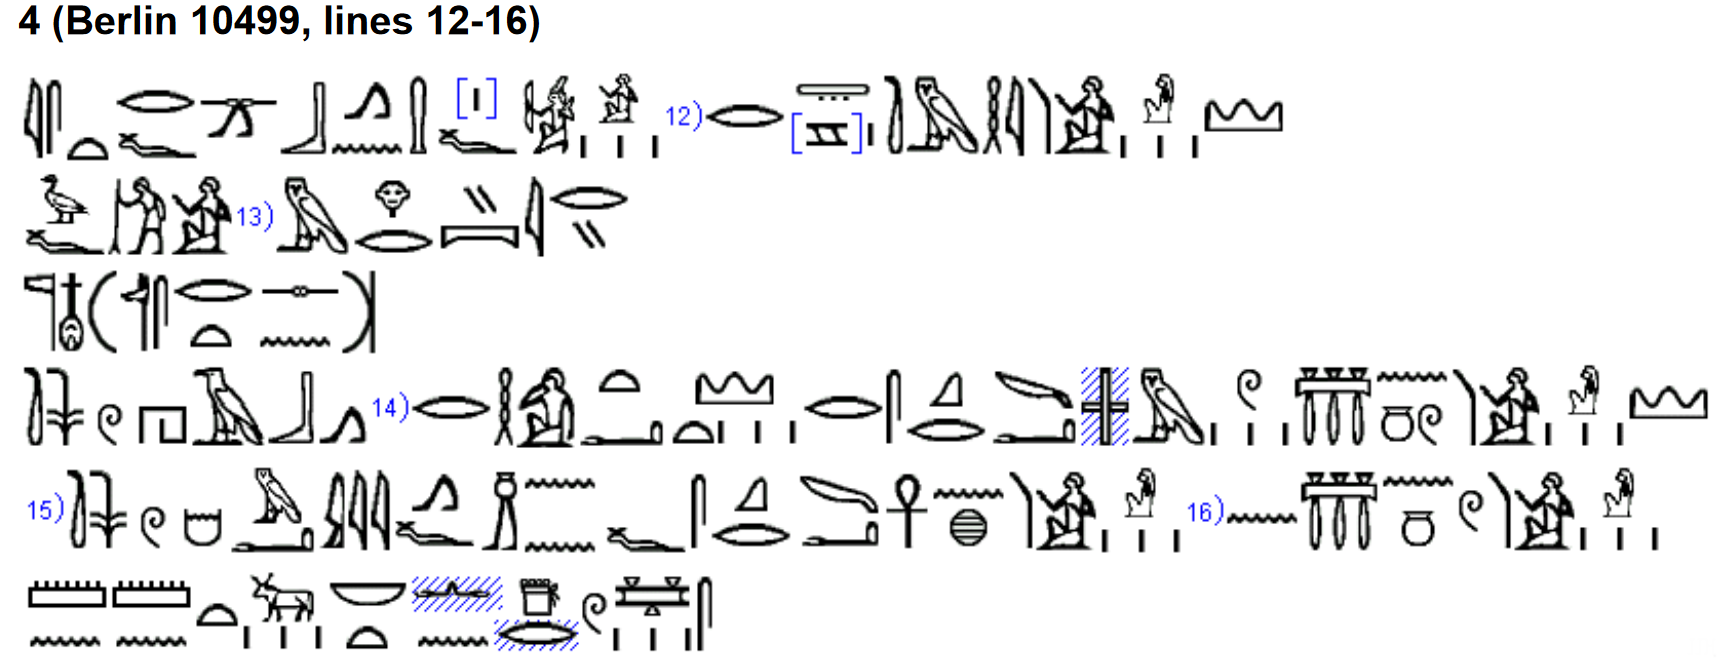
\includegraphics[width=1.0\textwidth]{hiero_1.PNG}
%http://carrington-arts.com/JJSinuhe/Sinuhe.pdf
\paragraph{}~\\
Will the tool be able to:
\newline ~\\
\begin{itemize}  
\item Generate a readable facsimile from a source image?
\item Identify individual signs correctly?
\item Identify groupings of signs correctly?
\item Provide accurate information on the meaning of these signs and groupings?
\item Provide accurate information on the potential transliteration of the text?
\end{itemize}
\paragraph{} ~\\ \noindent \textbf{Challenges:}
\newline \break \noindent
There isn't a lot of documentation on what this tool can and cannot do, so this will actually be an exercise in figuring that out.
\newline \break \noindent
Any pitfalls that the tool suffers from cannot be known yet, as it is not widely documents or available for use yet.
\newline \break \noindent
There is no way of knowing what the pitfalls and limitations of the tool are without being able to test it
\newline \break \noindent
I will not be able to test any of these issues or steps until I gain access to the tool itself.
\newline \break \noindent
To what extent does it actually assist in the process of translating hieroglyphs
\newline \break \noindent
What do I want it to do? Provide information along the way - be able to be interacted with in order to determine what the signs and group signs are, which will lead to a transliteration, then provide interactive dictionary tools to create a translation.
\newline \break \noindent
Are there examples of this being done? Not that I know of, at least not specifically using the Hieroglyphics Initiative itself. There are older programs that were used in hieroglyph translation: Glyph, WinGlyph, MacScribe, Inscribe, VisualGlyph, VectorOffice and Hieroglyphica.

%Gozzoli, R. (2013), ‘Hieroglyphic Text Processors, Manuel de Codage, Unicode, Lexicon,’ in S. Polis, and J. Winand (eds.), Technology, Texts, Languages and Information Technology in Egyptology, Selected papers from the meeting of the Computer Working Group of the International Association of Egyptologists (Informatique & Égyptologie), Presses Universitaires de Liège, Liège, 89-101. 

\end{document}